% Formatting
\documentclass[]{book}
\usepackage[margin = 1in, paperwidth = 6in, paperheight = 9in,twoside]{geometry}
\usepackage{microtype}
\usepackage{multicol}
\usepackage{makeidx}
\makeindex

% Graphics
\usepackage{graphicx}

% Math Packages
\usepackage{amsmath}
\usepackage{amsthm}
\newtheorem{theorem}{Theorem}[chapter]
\newtheorem{corollary}{Corollary}[theorem]
\newtheorem{lemma}[theorem]{Lemma}
% Boldface Proof
\makeatletter
\renewenvironment{proof}[1][\proofname] {\par\pushQED{\qed}\normalfont\topsep6\p@\@plus6\p@\relax\trivlist\item[\hskip\labelsep\bfseries#1\@addpunct{.}]\ignorespaces}{\popQED\endtrivlist\@endpefalse}
\makeatother

\newlength{\mylen}
\setbox1=\hbox{$\bullet$}\setbox2=\hbox{\tiny$\bullet$}
\setlength{\mylen}{\dimexpr0.5\ht1-0.5\ht2}

% Pseudocode Verbatim Environment
\usepackage{fancyvrb}
\renewcommand{\theFancyVerbLine}{%
 {\small\arabic{FancyVerbLine}}}  % line numbers
 \fvset{numbers=left,xleftmargin=10mm}

% Table of Contents custom package
\usepackage{tocloft}
\usepackage[nottoc]{tocbibind}
% Removes dots from ToC
\renewcommand{\cftdot}{}
% Customizes fonts for ToC; removes dots; changes style of text and indentation
\renewcommand{\cfttoctitlefont}{\LARGE\bfseries\MakeUppercase}
\renewcommand{\cftchapfont}{\Large\bfseries}
\renewcommand{\cftchappagefont}{\bfseries}
\renewcommand{\cftsecpresnum}{\bfseries}
\renewcommand{\cftchapaftersnum}{.}
\renewcommand\cftchapafterpnum{\vskip 10pt}
\setlength{\cftchapnumwidth}{25pt}
\setlength{\cftsecindent}{25pt}
\setlength{\cftsubsecindent}{50pt}
\setlength{\cftbeforechapskip}{15pt}
\normalsize{\settocbibname{References}}
\normalsize{\setindexname{Index}}

% Responsible for removing headings off clear pages
\makeatletter
\renewcommand*{\cleardoublepage}{\clearpage\if@twoside \ifodd\c@page\else
\hbox{}%
\thispagestyle{empty}%
\newpage%
\if@twocolumn\hbox{}\newpage\fi\fi\fi}
\makeatother

% Title page
\author{}
\title{}
\date{}

% Macros
\newcommand{\runtime}[1]{\textbf{Running time:} $O(#1)$\\}
\newcommand{\memory}[1]{\textbf{Memory space:} $O(#1)$\\}

% hyperref must be the last command in preamble
\usepackage[pdftex]{hyperref}

\begin{document}
  \frontmatter
  \thispagestyle{empty}
  \begin{center}
    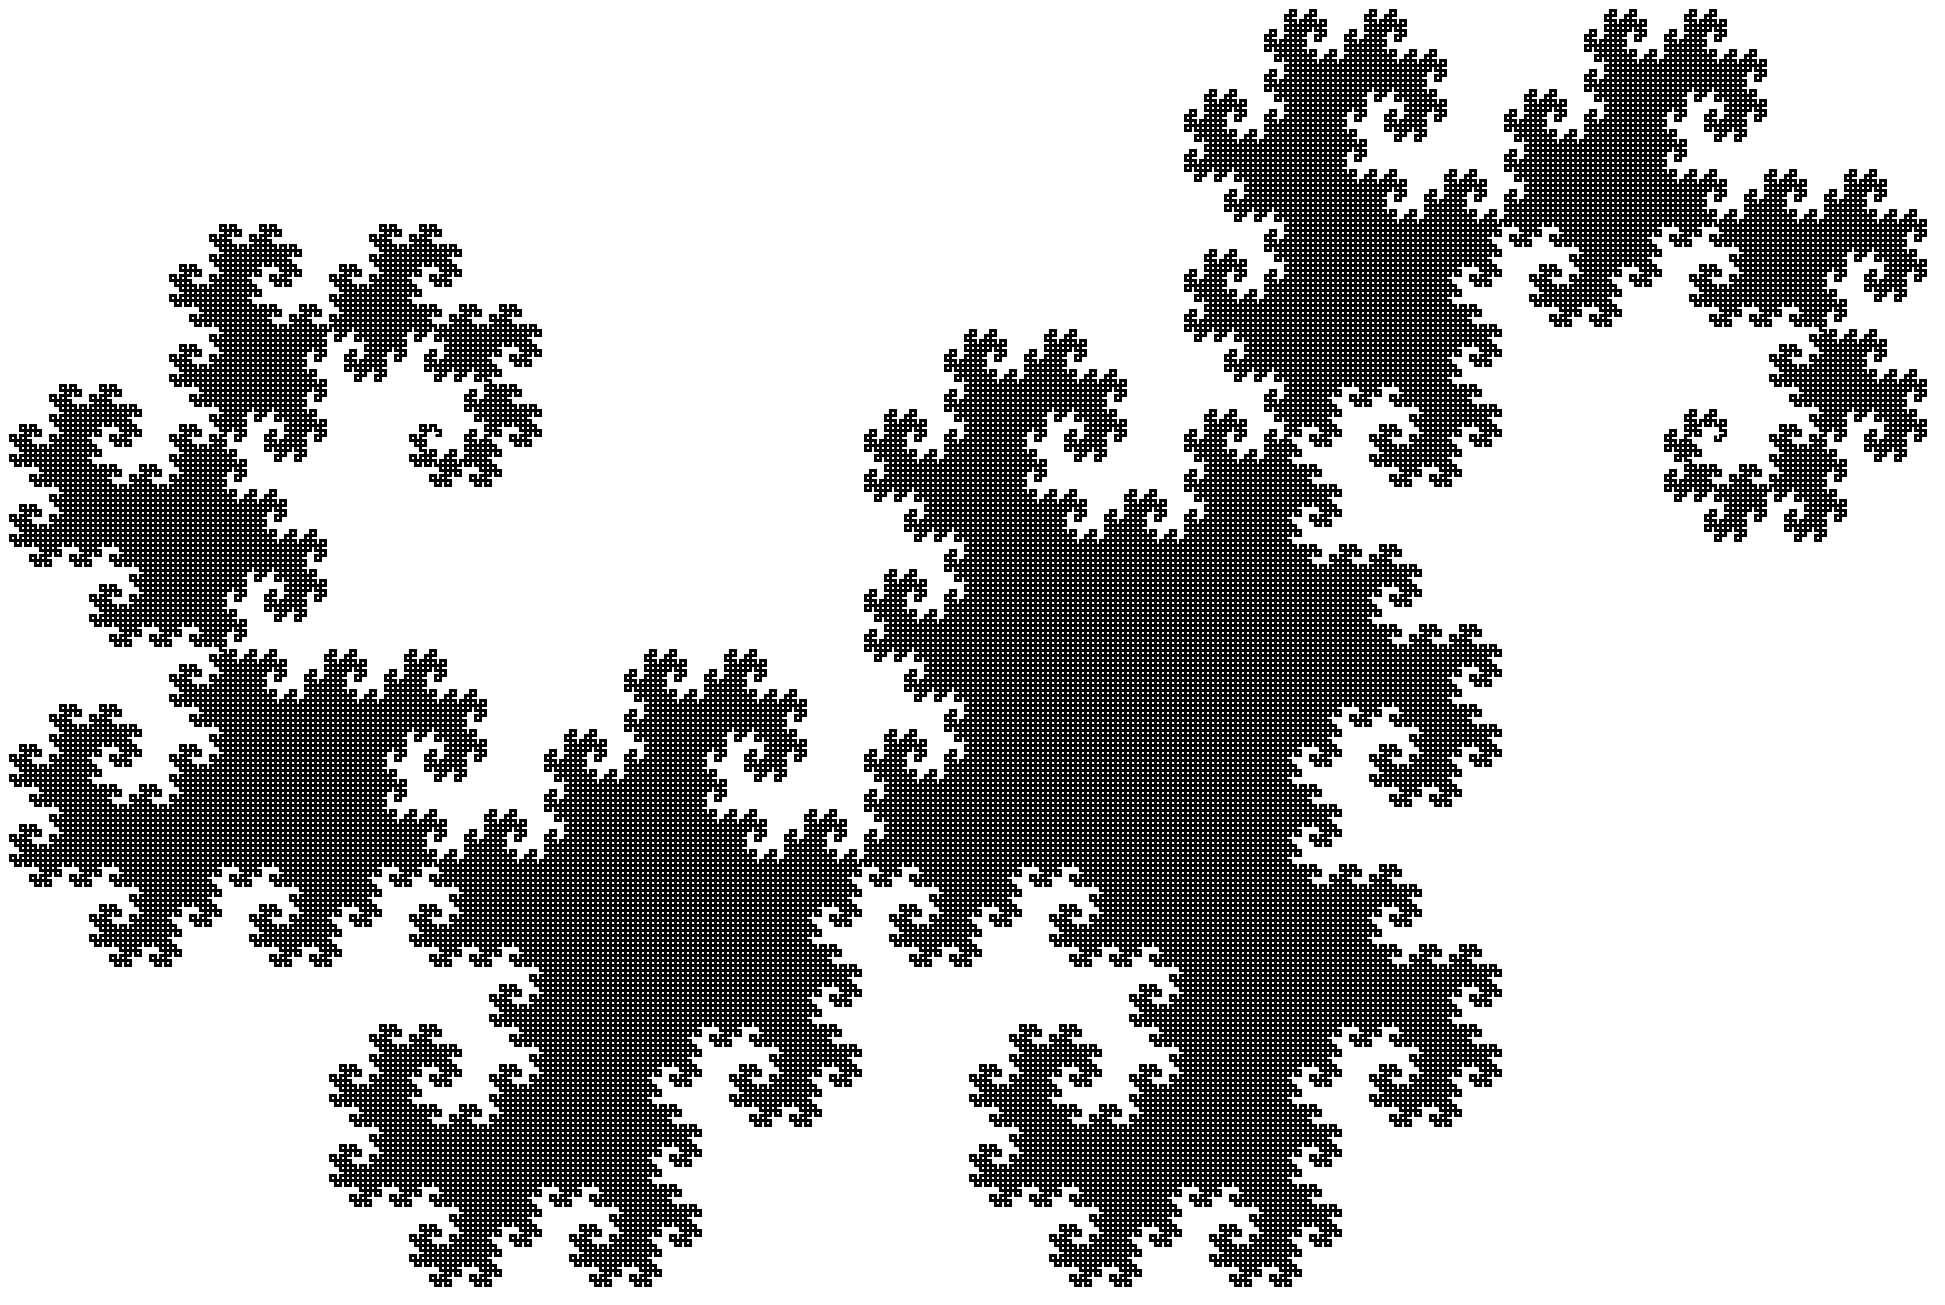
\includegraphics[scale=0.17]{dragon16.png}
  \end{center}
  \clearpage
  \newgeometry{margin = 1in, top=0.75in, paperwidth = 6in, paperheight = 9in,twoside} %customize margins for special pages
  \tableofcontents
  \thispagestyle{empty}

  \chapter*{Preface}
    \indent Some competition environments allow texts with a certain criterea. ICPC\index{ICPC} World Finals
    rules that a team may bring a \textbf{Team Reference Document}, a document containing up to
    25 pages of reference materials, single-sided, letter or A4 size. This manual does not
    follow the requisite, but it is written as a lightweight reference material.\\
    \indent When I first started preparing for prgroamming contests, I started off solving
    problems on sites like CodeForces, SPOJ, TopCoder, etc. However, what I learned was
    that knowing a bunch of solutions to particular problems isn't useful if you don't understand
    the theory of why they work and the many possible variations each problem provides. You won't
    be able to use the properties of algorithms for problems if you haven't studied the algorithms
    themselves.\\
    \indent I originally wanted to include theorems and proofs of correctness, but there wasn't
    enough time, so I highly suggest you read CLRS\index{CLRS} for proofs and theory. We believe
    proof of correctness is important, but those can be found in other textbooks. Our primary focus
    is to implement and design algorithms for particular problems. You can think of this
    text as a ``cookbook'' for algorithms.\\
    \indent We have included an two appendixes. Appendix 1 is devoted to common data structures we
    encountered using Java and C++. Appendix 2 includes common mathematical formulas for reference.
    \restoregeometry  %Restore to original margins

  \mainmatter
  \chapter{Asymptotic Notation}
    \section{$\Theta$-notation}
      $\Theta$-notation asymptotically bounds a function from above and below. It expresses
      the worst case running time of a given function. For a given function $g(n)$, we denote
      $\Theta(g(n))$ as the \textit{set of functions}
      \begin{multline*}
        \theta(g(n)) = f(n): \text{there exist positive constants}\ c_1\ c_2 \text{and}\ n_0\\
        \text{such that}\ 0 \leq c_1g(n) \leq f(n) \leq c_2g(n) \text{for all}\ n\geq n_0
      \end{multline*}
      A function $f(n)$ belongs to the set $\Theta(g(n))$ if there exists positive constants
      $c_1$ and $c_2$ such that it can be ``sandwiched'' between $c_1g(n)\ \text{and}\ c_2g(n)$ for
      sufficiently large $n$. $g(n)$ is an \textbf{asymptotically tight bound} \index{asymptotic!tight bound}for $f(n)$.
    \section{$\mathcal{O}$-notation}
      We use $O$-notation when we only have an \textbf{asymptotic upper bound}\index{asymptotic!upper bound}.
      For a given function $g(n)$, we denote by $O(g(n))$ the set of functions
      \begin{multline*}
        O(g(n))=f(n):\ \text{there exists positive constants}\ c\ \text{and}\ n_0\\
        \text{such that}\ 0 \leq f(n) \leq cg(n) \text{for all}\ n \geq n_0.
      \end{multline*}
      We write $f(n) = O(g(n))$ to indicate that a function $f(n)$ is a member of
      the set $O(g(n))$. Note that $f(n) = \Theta(g(n))$ which implies $f(n) = O(g(n))$ since
      $\Theta$-notation is a stronger notation than $O$-notation.
    \section{$\Omega$-notation}
      Just as $O$-notation provides an asymptotic \textit{upper} bound on a function,
      $\Omega$-notation provides an \textbf{asymptotic lower bound} \index{asymptotic!lower bound}for $f(n)$.
      \begin{multline*}
        \Omega(g(n)) = f(n):\ \text{there exists positive constants}\ c\ \text{and}\ n_0\\
        \text{such that}\ 0 \leq c(g(n)) \leq f(n)\ \text{for all}\ n \geq n_0.
      \end{multline*}

    \begin{theorem}
      For any two functions $f(n)$ and $g(n)$, we have $f(n) = \Theta(g(n))$
      if and only if $f(n) = O(g(n))$ and $f(n) = \Omega(g(n))$.
    \end{theorem}

    \section{$o$-notation}
      $o$-notation is defined as not asymptotically tight in upper bound.
      \begin{multline*}
        o(g(n)) = f(n): \text{for any positive constant}\ c > 0,\ \text{there exists}\\\text{ a constant}\
        n_0 > 0\ \text{such that}\ 0 \leq f(n) < cg(n)\ \text{for all}\ n \geq n_0.
      \end{multline*}
      Intuitively, in $o$-notation the function $f(n)$ becomes insignificant relative
      to $g(n)$ as $n$ approaches infinity.
      $$\lim_{n\to\infty} \dfrac{f(n)}{g(n)} = 0$$
      If $f(n)$ was asymptotically tight, then the limit would approach 1.

    \section{$\omega$-notation}
      $\omega$-notation is to $\Omega$-notation as $o$-notation is to $O$-notation. $\omega$-notation
      is used to denote a lower bound that is not asymptotically tight.
      \begin{multline*}
        \omega(g(n)) = f(n): \text{for any positive constant}\ c > 0,\ \text{there exists}\\\text{ a constant}\
        n_0 > 0\ \text{such that}\ 0 \leq cg(n) < f(n) \text{for all}\ n \geq n_0.
      \end{multline*}
      The relation $f(n) = \omega(g(n))$ implies that $$\lim_{n\to\infty} \dfrac{f(n)}{g(n)} = \infty$$
      if the limit exists.

    \section*{Comparing functions}
      Many relational properties of real numbers also apply to asymptotic comparisons.
      \subsection*{Transitivity}
  \chapter{Divide and Conquer}
    In divide-and-conquer, we solve a problem recursively, applying three steps
    at each level of recursion.\\

    \noindent\textbf{Divide} the problem into a number of subproblems that are smaller instances of the same problem.\medskip\\
    \textbf{Conquer} the subproblems by solving them recursively. If the subproblem sizes are small enough, just solve the subproblems
    in a straightforward manner.\medskip \\
    \textbf{Combine} the solutions to the subproblems into the solution for the original problem.

      \subsection*{Recurrences}
        Recurrences give us a natural way to characterize the running times of divide-and-conquer algorithms.
        A \textbf{recurrence} is an equation or inequality that describes a function in terms of its value
        on smaller inputs.
        CLRS provides three methods for obtaining an asymptotic ``$\Theta$'' or ``$\mathcal{O}$'' bounds:
        \renewcommand\labelitemi{\raisebox{\mylen}{\tiny$\bullet$}}
        \begin{itemize}
          \item substitution method
          \item recursion-tree method
          \item the master method
        \end{itemize}
    \section{Substitution}
      In the substitution method, we guess a bound and then use mathematical
      induction to prove our guess is correct.

    \section{Recursion-Tree}
      Drawing out a recursion tree serves as a straightforward way to devise
      a good guess. Each node represents the cost of a single subproblem. We
      sum up the costs within each level of the tree to obtain a set of per-level
      costs, then sum the per-level costs to determine total cost of the recurrence.

      Consider the recurrence $T(n) = 3T(\lfloor \frac{n}{4} \rfloor) + \Theta(n^2)$.
      We create a recursion tree for the recurrence $T(n) = 3T(n/4) + cn^2$.

    \section{Master's Theorem}
      The master method solves recurrences of the form
      \begin{flushleft}
        $T(n) = aT(n/b) + f(n)$
      \end{flushleft}
      where $a \geq 1$ and $b > 1$ are constants and $f(n)$ is an asymptotically positive
      function. $T(n)$ has the following asymptotic bounds:
      \begin{enumerate}
        \item If $f(n) = O(n^{\log_b a-\epsilon})$ for some constant $\epsilon > 0$,
        then\medskip\\ $T(n) = \Theta(n^{\log_b a})$.
        \item If $f(n) = \Theta(n^{\log_b a})$, then $T(n) = \Theta(n^{\log_b a}\lg n)$.
        \item If $f(n) = \Omega(n^{\log_b a+\epsilon})$ for some constant $\epsilon > 0$, and if
        $af(n\b) \leq cf(n)$ for some constant $c < 1$ and all sufficiently large $n$, then
        $T(n) = \Theta(f(n))$.
      \end{enumerate}
  \chapter{Quicksort}
    Quicksort, like merge sort applies the divide-and-conquer paradigm.
  \chapter{Trees}

  \chapter{Graphs}
  You might know that both DFS and BFS explore an unweighted graph. But why does one use DFS
  and not BFS in Kosaraju's strongly connected components algorithm? Dijkstra's algorithm assumes
  nonnegativity, but why can one sometimes use Dijkstra's when some weights are negative?

  Graphs are a fundamental data structure in the world of programming. Formally
  a \textbf{graph}\index{graph} G consists of a finite nonempty set V of objects called \textbf{vertices}
  and a set E called \textbf{edges}. G is an ordered pair of sets V and E. $$ G = (V,E)$$
  \indent Graphs are often used to represent physical entities (a network of roads, relationship
  between people). Common graph problems include shortest paths, number of minimum cuts,
  strongly connected components \ldots.

    \section{Breadth-First Search}
    \indent Often labeled as a `cautionary search', the plan of \textbf{Breadth-First Search}
    is to uniformally explore the nodes of a graph outwards. In BFS, we pick a starting node
    $n_1$ and visit all of $n_1$'s neighbors before visiting their neighbors.\\
    \indent The main perk of BFS over other search algorithms is it can compute shortest
    paths\index{shortest path} in unweighed graphs\index{unweighed graph}.
    \begin{Verbatim}
void search(Node root){
  queue.add(root);
  visited.add(root);
  level = 0;
  while(!queue.empty())
  {
    Node index = queue.pop();
    for each (Node n in index.adjacent)
    {
      if (n.visited == false)
      {
        level = index.level+1;
        visited.add(n);
        queue.add(root);
      }
    }
  }
}
    \end{Verbatim}
    \runtime{V + E}

      \subsection*{Bipartite Graph}
      We define a graph as \textbf{bipartite}\index{bipartite} graphs if $V(G)$ can be partitioned into two
      subsets $U$ and $W$ such that every edge of G joins a vertex of $U$ and a vertex of $W$. We can
      determine if a graph is bipartite using BFS.
      \begin{enumerate}
        \item Run BFS from any node $u$.
        \item If we encounter a previously visited node $v$, we should check if $u$ and $v$ are both
        even or both odd. If either of these conditions hold, then the graph is not bipartite.
      \end{enumerate}

      \subsection*{Diameter of Tree}\index{diameter}
      \begin{enumerate}
        \item Run BFS from any node to find the farthest leaf node. Label that node T.
        \item Run another BFS to find farthest node from T.
      \end{enumerate}
      \begin{proof}
        Let us assume that the diameter of the graph is unique. That is, there exists exactly
        one pair of vertices ${u,v}$ which is the highest path length among any pair of vertices.
        First, we establish that $u$ and $v$ must be leaf nodes, otherwise, there exists a
        longer highest path.

        Take any node $w$ and find the vertex which is furthest from it. We will show that the vertex
        found will be either $u$ or $v$. Suppose that the vertex found is different, say $z$.
        Consider two cases:\\

        \underline{Case 1:} $w$ lies on the path from $u$ to $v$.\\
        Without loss of generality, let the $w-u$ path have no edges overlapping with the $w-z$ path.
        The distance from $w$ to $z$ is greater than $w$ to $u$ and $w$ to $v$. If true, then
        $d(u,z) = d(u,w) + d(w,z) \geq d(u,w) + d(w,v) = d(u,v)$. This contradicts the assumption that
        $d(u,v)$ is the unique diameter of the tree.\\

        \underline{Case 2:} $w$ does not lie on the path from $u$ to $v$.\\
        Now, either the $w-z$ path either overlaps with $u-v$ path or is disjoint. If there is overlap,
        let $y$ be the vertex closest to w among the overlapped vertices. The distance from $y$ to $z$
        must be greater than $y$ to $v$. Hence $d(u,z) = d(u,y) + d(y,z) \geq d(u,y) + d(y,v) = d(u,v)$.
        This once again contradicts the assumption of ${u,v}$ being the unique diameter of the tree.\\

        If the paths do not overlap, there are vertices $x$ and $y$ on the $u-v$ and $w-z$ paths
        respectively wich are closest to each other. $d(y,z) \geq d(y,v)$. Hence $d(u,z) = d(u,y) + d(y,z)
        \geq d(u,y) = d(y,v) > d(u,x) + d(x,v) = d(u,v)$. Hence the assumption that d(u,v) is the diameter
        is contradicted.\\

        We see that in each case, there is a contradiction if $z$ is not one of $u$ or $v$. Hence it follows
        that $z$, the furthest vertex from $w$, is either $u$ or $v$.
      \end{proof}

    \section{Depth-First Search}
    If BFS is the cautious and tentative exploration strategy, then \textbf{Depth-First Search}
    \index{DFS}(DFS) is its more aggressive cousin. DFS explores aggressively, delving deeper
    into the graph and backtracks only when necessary.\\
    \indent The implementation of DFS is similar to BFS, but instead of using a queue\index{queue}, we
    use a stack\index{stack}. Another method is to use recursion\index{recursion}.\\
    \begin{Verbatim}
void search(Node root){
  if(root == null) return;
  visit(root);
  root.visited = true;
  for each (Node n in root.adjacent) {
    if (n.visited == false) {
      search(n);
    }
  }
}
    \end{Verbatim}
    \runtime{V + E}
    Why use DFS over BFS? DFS has its own catalog of applications that can't be replicated
    using BFS.
    \begin{itemize}
      \item Computing a topological ordering of directed acyclic graphs
      \item Computing strongly connected components of directed graphs
    \end{itemize}

      \subsection*{Topological Sort}
      A \textbf{topological ordering}\index{topological ordering} of a directed graph G
      is a labeling $f$ of G's nodes such that:
      \begin{enumerate}
        \item the $f(v)$'s are the set ${1,2,\ldots, n}$
        \item $(u,v) \in G \Rightarrow f(u) < f(v)$
      \end{enumerate}

      As long as our structure is a directed acyclic graph (DAG), we can compute a topological ordering.
      Every DAG has a sink vertex. Remove the sink vertex, and the remaining graph is a DAG. (Unless
      $|v| < 1$) The pseudocode for a topological sort is as follows:
      \begin{Verbatim}
DFS(graph G, start vertex s) {
  visit(s);
  for each edge (s,v) {
    if(v.visited == false)
      DFS(G, v);
  }
  set f(s) = current_label
  current_label--;
}

topologic_sort(graph G) {
  mark all nodes unexplored;
  current_label = n;
  for each vertex v of G {
    if(v.visited == false)
      DFS(G, v);
  }
}
      \end{Verbatim}
      \runtime{V + E}
      \memory{V + E}
      \begin{proof}
        Take any edge, $(u,v)$. We will show that $f(u) < f(v)$.\\

        \underline{Case 1:} u is visited by DFS before v\\
        u will recursively call v, which will continue DFS. Eventually v will exhaust
        its adjacent neighbors and become a sink vertex before u. $f(u) < f(v)$\\

        \underline{Case 2:} v is visited by DFS before u\\
        v makes recursive DFS calls. u will never be visited during these recursively calls,
        otherwise the graph would contain a directed cycle. As a result, v will become a sink
        vertex before u is visited. $f(u) < f(v)$
      \end{proof}

      \subsection*{Strongly Connected Components}
      The \textbf{strongly connected components}\index{SCC} of a directed graph G are defined
      as the equivalence classes of the relation $u\sim v \Leftrightarrow \exists$ path$(u,v)$ and
      path$(v,u)$. SCCs can be computed using \textbf{Kosaraju's Two Pass algorithm}
      \index{Kosaraju}.

      The idea behind Kosaraju's algorithm is to perform two-DFS. The first DFS provides a topological
      sort. We then reverse the direction of each edge in $G$, yielding $G'$. $G$ and $G'$ contain
      the same amount of strongly connected components, so we perform DFS once again, this time
      with a specific ordering obtained by our topological sort.

      Kosaraju's Two Pass Algorithm:
      \begin{verbatim}
// Credit to geeksforgeeks.org
// C++ Implementation of Kosaraju's algorithm to print all SCCs
#include <iostream>
#include <list>
#include <stack>
using namespace std;

class Graph
{
	int V; // No. of vertices
	list<int> *adj; // An array of adjacency lists

	// Fills Stack with vertices (in increasing order of finishing
	// times). The top element of stack has the maximum finishing
	// time
	void fillOrder(int v, bool visited[], stack<int> &Stack);

	// A recursive function to print DFS starting from v
	void DFSUtil(int v, bool visited[]);
public:
	Graph(int V);
	void addEdge(int v, int w);

	// The main function that finds and prints strongly connected
	// components
	void printSCCs();

	// Function that returns reverse (or transpose) of this graph
	Graph getTranspose();
};

Graph::Graph(int V)
{
	this->V = V;
	adj = new list<int>[V];
}

// A recursive function to print DFS starting from v
void Graph::DFSUtil(int v, bool visited[])
{
	// Mark the current node as visited and print it
	visited[v] = true;
	cout << v << " ";

	// Recur for all the vertices adjacent to this vertex
	list<int>::iterator i;
	for (i = adj[v].begin(); i != adj[v].end(); ++i)
		if (!visited[*i])
			DFSUtil(*i, visited);
}

Graph Graph::getTranspose()
{
	Graph g(V);
	for (int v = 0; v < V; v++)
	{
		// Recur for all the vertices adjacent to this vertex
		list<int>::iterator i;
		for(i = adj[v].begin(); i != adj[v].end(); ++i)
		{
			g.adj[*i].push_back(v);
		}
	}
	return g;
}

void Graph::addEdge(int v, int w)
{
	adj[v].push_back(w); // Add w to v’s list.
}

void Graph::fillOrder(int v, bool visited[], stack<int> &Stack)
{
	// Mark the current node as visited and print it
	visited[v] = true;

	// Recur for all the vertices adjacent to this vertex
	list<int>::iterator i;
	for(i = adj[v].begin(); i != adj[v].end(); ++i)
		if(!visited[*i])
			fillOrder(*i, visited, Stack);

	// All vertices reachable from v are processed by now, push v
	Stack.push(v);
}

// The main function that finds and prints all strongly connected
// components
void Graph::printSCCs()
{
	stack<int> Stack;

	// Mark all the vertices as not visited (For first DFS)
	bool *visited = new bool[V];
	for(int i = 0; i < V; i++)
		visited[i] = false;

	// Fill vertices in stack according to their finishing times
	for(int i = 0; i < V; i++)
		if(visited[i] == false)
			fillOrder(i, visited, Stack);

	// Create a reversed graph
	Graph gr = getTranspose();

	// Mark all the vertices as not visited (For second DFS)
	for(int i = 0; i < V; i++)
		visited[i] = false;

	// Now process all vertices in order defined by Stack
	while (Stack.empty() == false)
	{
		// Pop a vertex from stack
		int v = Stack.top();
		Stack.pop();

		// Print Strongly connected component of the popped vertex
		if (visited[v] == false)
		{
			gr.DFSUtil(v, visited);
			cout << endl;
		}
	}
}
      \end{verbatim}
  \chapter{Weighted Graphs}
  \chapter{Numbers}
    \section{Primes}
      \subsection*{Generating Prime Table}

  \chapter{Hash Tables}
    Comparing arrays and linked lists, we learned that arrays are able to search for an element
    in $O(1)$. Linked lists on the other hand takes $\Theta(n)$ time in the worst case.

    A hash table generalizes the simpler notion of an ordinary array using \textit{direct addressing}. \index{direct addressing}
    Direct addressing allows us to examine an arbitrary position in an array in $O(1)$ time. In
    hash tables, the array index is \textit{computed} from the key.

    \section{Direct-address tables}
      Direct addressing works well when the universe $U$ of keys is reasonably small.
      Suppose we have a dynamic set where each element has a key drawn from the universe $U = \left\{ 0,1, \ldots, m - 1 \right\}$
      Assume no two elements have the same key.

  \chapter{Bitwise Operators}
    In low-level programming, it is often necessary to access memory locations and change individual bits.
    \textbf{Bitwise operators} provide a straightforward method to tinker with bits and bytes. There are
    scenarios when bitwise operators provide a simpler and quicker method over loops and recursion.
    \section{Bread and Butter Operators}
    % http://graphics.stanford.edu/~seander/bithacks.html#SwappingValuesSubAdd
    \subsection*{Bitwise Shifting}
    The leftshift operator is the equivalent of moving all the bits of a number a specified number of places to the left:
    \begin{verbatim}
      [variable] << [number_of_places]
    \end{verbatim}
    For instance, consider the number 8 written in binary 00001000. If we wanted to shift it to the left 2 places, we'd end up with
    00100000; everything is moved to the left two places, and zeros are added as padding. This is the number 32.

    Essentially left shifting is the equivalent of multiplying by a power by two. Just as there is a left shift operator, there also exists
    the right shift operator (\textgreater\textgreater).
    \pagebreak

    \subsection*{Bitwise AND}
    The bitwise AND operator is a single ampersand. A binary AND takes the logical AND of the bits
    in each position of a number in binary form. \textbf{Example}: 72 \& 184 = 8
    \begin{verbatim}
      01001000 &
      10111000 =
      --------
      00001000
    \end{verbatim}

    \subsection*{Bitwise OR}
    The bitwise OR operator symbol is a single pipe: $\vert$. Only one of the two bits must be true to return true
    for that position's bit. \textbf{Example}: 72 $\vert$ 184 = 248
    \begin{verbatim}
      01001000 |
      10111000 =
      --------
      11111000
    \end{verbatim}

    \subsection*{Bitwise Complement}
    The bitwise complement operator, the tilde $\sim$, flips every bit.
    This turns out to be a great way of finding the largest possible value for an unsigned number:
    \begin{verbatim}
      unsigned int max = ~0;
    \end{verbatim}

    \subsection*{Bitwise XOR}
    The exclusive-or operator takes two inputs and returns a 1 if either one or the other of the
    inputs is a 1, but not if both are. The symbol for XOR is $\wedge$.
    \begin{verbatim}
      01110010 ^
      10101010 =
      --------
      11011000
    \end{verbatim}
    \pagebreak

    Using bitwise operators are good for saving space and time when used properly. Here are a couple
    examples:\\\\
    \textbf{Checking if a number is a power of 2}:
    \begin{verbatim}
    n & (n-1) == 0
    \end{verbatim}
    \textbf{Checking if a number is of form $2^n-1$}:
    \begin{verbatim}
    n & (n+1) == 0
    \end{verbatim}
    \textbf{Checking if the rightmost bit is set}:
    \begin{verbatim}
      n & 1 == 1
    \end{verbatim}
    \textbf{Round up to next highest power of 2}
    \begin{Verbatim}
unsigned int v;

v--;
v |= v >> 1;
v |= v >> 2;
v |= v >> 4;
v |= v >> 8;
v |= v >> 16;
v++;
    \end{Verbatim}
    \textbf{Reverse bits}
    \begin{Verbatim}
unsigned int v;     // input bits to be reversed
unsigned int r = v; // r will be reversed bits of v
int s = sizeof(v) * CHAR_BIT - 1; // extra shift needed at end

for (v >>= 1; v; v >>= 1)
{
  r <<= 1;
  r |= v & 1;
  s--;
}
r <<= s; // shift when v's highest bits are zero
    \end{Verbatim}
    \section{Bit Masking}
    The process of masking is similar to preparing to spray paint an object. You want to cover any exposed areas
    so that the spray paint is applied to the object barring the covered area. Bit masking is the act of applying
    a mask to a value via bit operations. \\\\
    \textbf{Determining if a number is a power of four}:
    \begin{verbatim}
(num & 1 == 0) and (num & num-1) == 0 and (num & 0xAAAAAAAA == 0);
    \end{verbatim}
    The hexadecimal value of 0xAAAAAAAA acts as a mask for 1010 1010 1010 1010 1010 1010 1010 1010 in binary.

  \backmatter
  \setlength{\cftbeforechapskip}{15pt}
  \renewcommand\cftchapafterpnum{\vskip 10pt}
  \renewcommand\bibname{\large{References}}
  \newgeometry{margin = 1in, top=0.25in, paperwidth = 6in, paperheight = 9in,twoside}
  \begin{thebibliography}{9}
  \bibitem{latexcompanion}
  Michel Goossens, Frank Mittelbach, and Alexander Samarin.
  \textit{The \LaTeX\ Companion}.
  Addison-Wesley, Reading, Massachusetts, 1993.

  \bibitem{einstein}
  Albert Einstein.
  \textit{Zur Elektrodynamik bewegter K{\"o}rper}. (German)
  [\textit{On the electrodynamics of moving bodies}].
  Annalen der Physik, 322(10):891–921, 1905.

  \bibitem{knuthwebsite}
  Knuth: Computers and Typesetting,
  \\\texttt{http://www-cs-faculty.stanford.edu/\~{}uno/abcde.html}
  \end{thebibliography}

  %\bibitem{graphtheory}
  %Chartrand, Gary, and Ping Zhang.
  %\textit{A First Course in Graph Theory}.
  %Dover Publications, Mineola, New York, 2012. Print.

  \appendix
  \chapter{\large{Appendix I: \textnormal{Data Structures}}}
  \chapter{\large{Appendix II: \textnormal{Mathematical Formulae}}}
  \printindex
\end{document}
